\chapter{Symulacja dynamiki płynów i przewodnictwa cieplnego jako wartościowe narzędzie edukacyjne}

\en jest interaktywną, edukacyjną symulacją, która modeluje mechanizmy
przekazywania ciepła w przyrodzie takie jak przewodnictwo cieplne oraz
konwekcja. Ponadto, możliwe jest również modelowanie zagadnień związanych z
szeroko pojętą dynamiką płynów.

Uczniowie i studenci mogą używać symulatora \en jako narzędzia, które pozwala
eksplorować przepływ ciepła i masy w dwuwymiarowych strukturach. Możliwa jest
bardzo szeroka konfiguracja warunków symulacji dzięki czemu można modelować
różnorodne, rzeczywiste obiekty (stworzone z materiałów o określonej pojemności
cieplnej i dowolnych kształtach) oraz warunki środowiskowe takie jak np. wiatr.
Nauczyciele fizyki, przyrody czy też przedmiotów ściśle inżynieryjnych, od
nauczania podstawowego po akademickie, mogą odkryć w \en wartościowe wsparcie
swoich zajęć edukacyjnych. Symulacja umożliwia prezentacje złożonych, naukowych
bądź też inżynieryjnych koncepcji bez sięgania po trudne wyrażenia matematyczne.

\en działa w natywnym środowisku przeglądarki internetowej, nie wymagając przy
tym instalowania żadnych rozszerzeń. Jest to złożona aplikacja, jednak w pełni
napisana w języku \js wspieranym przez praktycznie każdą dostępną obecnie
przeglądarkę. W pełni korzysta z najnowszych osiągnięć technologii internetowych
takich jak HTML5 oraz WebGL. Ponadto, dbając o jak najszerszą dostępność dla
użytkowników, silniki fizyczne zostały zaimplementowane w dwóch wersjach:

\begin{itemize} 

\item Wyłącznie w języku \js, co oczywiście oznacza, że obliczenia wykonywane są
na procesorze głównym komputera.

\item Przy użyciu języka \js oraz nowoczesnej technologii \ow{WebGL}, dzięki
czemu możliwe stało się przeniesienie wykonywania najbardziej wymagających
algorytmów fizycznych na procesor karty graficznej.

\end{itemize}

Obie wersje są ze sobą w pełni zgodne. Podwójna implementacja zapewnia doskonałą
optymalizację wydajnościową w przypadku, gdy konfiguracja sprzętowa oraz
oprogramowania wspiera nowoczesną technologię \ow{WebGL}. Z drugiej strony,
kiedy użytkownik dysponuje starszym komputerem bądź też starszą wersją
przeglądarki internetowej, wciąż ma możliwość używania aplikacji, która
automatycznie wykryje ten fakt i będzie wykorzystywać ,,zapasowe'' silniki
fizyczne napisane wyłącznie w \js.

Aplikacja powstała przy współpracy z amerykańską firmą The Concord Consortium,
która zajmuje się badaniami nad możliwościami poprawy jakości edukacji przy
użyciu najnowocześniejszych technologii. Jest ona oparta na innym symulatorze
stworzonym przez tę organizację, który był wykonany przy przy użyciu technologii
\ow{Java}. Obie wersje łączą zastosowania oraz algorytmy fizyczne opracowane
przez Charlesa Xie (przybliżone w sekcji \ref{sec:silnikiFizyczne}). Jednak nowa
wersja będąca przedmiotem tej pracy została napisana zupełnie od postaw ze
względu na odmienne środowisko wykonywania, użyte technologie oraz język
programowania. Różnice między środowiskiem Java, a środowiskiem JavaScript są
tak duże, że zupełnie różna jest też architektura aplikacji oraz oferowane
możliwości. Ponadto, wersja pierwotna w Javie umożliwiała wyłącznie sekwencyjne
obliczenia -- w przeciwieństwie do nowej wersji, na potrzeby której zostały
opracowane odpowiednie algorytmy równoległe.


\section{Możliwości symulatora}

Transfer ciepła jest zagadnieniem szeroko poruszanym podczas nauczania na
różnych etapach edukacji, szczególnie na lekcjach przyrody, ekologii czy też
fizyki. \en udostępnia szeroki wachlarz możliwości, który może uatrakcyjnić
tradycyjne lekcje oraz wykłady. Ponadto, stanowi doskonałą aplikację do
samodzielnych ćwiczeń. Uczeń sam może eksplorować wybrane zagadnienia w celu np.
uzyskania odpowiedzi na postawione pytania. Poniżej zaprezentowane jest
podsumowanie cech i możliwości symulatora \en:

\begin{description}

\item[Dwuwymiarowość.] Wizualizacje przedstawiają przekrój bądź też rzut sceny,
algorytmy fizyczne wykonują obliczenia na dwuwymiarowej siatce symulacyjnej.

\item[Interaktywność.] Obliczenia wykonywane są w czasie rzeczywistym,
z prędkością umożliwiającą zaobserwowanie rezultatów symulacji w krótkim
czasie po jej uruchomieniu.  

\item[Różnorodność wizualizacji.] Podstawowa wizualizacja symuluje obraz
kamery termowizyjnej, jednak jest możliwość prezentowania rozkładu temperatury
przy użyciu innych palet kolorów oraz skali szarości. Zakres prezentowych
temperatur również jest konfigurowalny.

\item[Elastyczność, szerokie możliwości konfiguracji.] Symulator opera się na
koncepcji przechowywania zserializowanych opisów scen w plikach w formacie
\ow{JSON} (powszechny format danych dla aplikacji \js). Plik konfiguracyjny
przechowuje informacje o:
\begin{itemize}

\item Warunkach brzegowych, takich jak ustalona temperatura bądź ustalony
przepływ ciepła.

\item Warunkach początkowych, takich jak wstępna temperatura różnych obiektów
na scenie.

\item Wszystkich obiektach na scenie oraz ich cechach, takich jak np. zdolność
do przewodzenia energii oraz pojemność cieplna.

\item Wymuszeniach, takich jak np. prędkość przepływu płynu w danym miejscu
(umożliwia symulację zjawisk związanych z dynamiką płynów oraz naturalnych
czynników środowiskowych takich jak wiatr).

\item Ustawieniach wizualizacji, takich jak paleta barw reprezentująca
wybrany zakres temperatur.

\item Ustawieniach symulacji, takich jak np. rozmiar siatki symulacyjnej, krok
czasowy symulacji oraz sugestia użycia równoległych algorytmów fizycznych
opierających się na technologii \ow{WebGL}.

\end{itemize} 

\item[Brak dodatkowych zależności i wymagań wobec przeglądarki internetowej.]
Aplikacja korzysta wyłącznie z języka \js oraz opcjonalnie z technologii
\ow{WebGL}, która jest częścią standardu \ow{HTML5}. Nie wymaga instalowania
żadnych dodatkowych rozszerzeń, nie stawia też wymagań wobec bibliotek i
narzędzi dostępnych w systemie (takich jak np. wirtualna maszyna Java).

\end{description}

\section{Motywacja i uzasadnienie osadzenia symulacji w środowisku przeglądarki internetowej}

Symulator \en z założenia był tworzony jako narzędzie edukacyjne. Doskonałym
miejscem gdzie może zostać użyty są wirtualne podręczniki nowej generacji.
Jednak te podręczniki, aby wnieść nową jakość w edukacji, powinny nie tylko
zostać bezpośrednio przeniesione z papieru na ekrany komputerów czy też innych
urządzeń elektronicznych, ale również wykorzystać w pełni ich możliwości.
Doskonałym medium rozpowszechniania takich podręczników jest internet oraz
strony HTML. Użytkownicy otrzymują łatwy, powszechny dostęp z każdego miejsca
oraz niewielkie wymagania wobec komputera i oprogramowania (dostęp do sieci oraz
przeglądarka internetowa to dziś praktycznie standard, szczególnie w szkołach).
Z kolei twórcy takich podręczników otrzymują bogate środowisko dla swoich
produktów, możliwość wprowadzenia interaktywności oraz wielu zaawansowanych
funkcji, a także łatwość aktualizacji oraz docierania do odbiorców.  Właśnie z
tego powodu symulator \en został osadzony w środowisku przeglądarki
internetowej. Również dlatego tak ważna była niezależność od zewnętrznych
technologii, rozszerzeń czy bibliotek -- zapewniło to brak niepotrzebnych
ograniczeń dostępności aplikacji dla użytkowników.

\en doskonale nadaje się do osadzenia w nowoczesnych źródłach wiedzy, ponieważ z
myślą o takim zastosowaniu została przeprowadzona cała implementacja. Osadzenie
aplikacji na stronie internetowej jest tak proste jak dodanie zwykłego obrazka
czy zdjęcia, gdyż symulacja wizualizowana jest na elementach HTML \ow{canvas}. W
praktyce wymagane jest dołączenie jednego pliku ze zbudowanym kodem \en oraz
wskazanie jednego kontenera \ow{div} w którym zostanie umieszczona symulacja.
Skalowanie i stylizowane tego kontenera zachowuje się zgodnie z przewidywaniami,
może do tego zostać użyta powszechnie znana technologia \ow{CSS} lub język \js.
Łatwość z jaką niezależni twórcy stron internetowych mogą użyć symulatora \en w
podręcznikach nowej generacji czy też wirtualnych laboratoriach, powoduje iż
aplikacja ta może mieć naprawdę szeroki wpływ na edukację.

\subsection{Obliczenia u klienta kontra obliczenia na serwerze}

Warto też zwrócić uwagę, iż przy wszelkich powyższych założeniach, w teorii
obliczenia związane z symulacją mogą być przeprowadzone w dwóch miejscach:

\begin{itemize} 

\item Na serwerze. Następnie wyniki muszą zostać przekazane za pośrednictwem
sieci do klienta w postaci np. danych, które byłby u niego wizualizowane bądź
też w postaci gotowego obrazu stanowiącego już wizualizację.

\item U klienta. Następnie wyniki również u klienta muszą zostać zwizualizowane.

\end{itemize}

Oba podejścia znajdują zastosowania w realnych zastosowaniach. Pierwsza metoda
jest dobra w przypadku bardzo czasochłonnych obliczeń, wykonywanych przez np.
superkomputer, kiedy wiele osób jest zainteresowanych wynikami jednego
eksperymentu czy też symulacji. Jednak biorąc pod uwagę wymagania stawiane przed
aplikacją \en, gdzie użytkowników mogą być tysiące i każdy z nich prawdopodobnie
uruchomi inną symulację, w innym momencie i nie jest zainteresowany wynikami
innych osób, takie podejście nie ma prawa zdać egzaminu. Nawet potężne serwery,
które uruchamiałyby tysiące niezależnych symulacji, prawdopodobnie nie byłyby w
stanie przesyłać obszernych wyników (używane siatki symulacyjne mają najczęściej
rozmiar 100x100 pól) z częstotliwością, która by zapewniła płynność symulacji
(minimum 30 wyników na sekundę). Również organizacja takiego zaplecza
sprzętowego prawdopodobnie stanowiłaby barierę finansową, która uniemożliwiłaby
powszechny dostęp do takiej aplikacji.

Obliczenia po stronie klienta rozwiązują całkowicie ten problem. Jako, że
symulacja nastawiona jest na interaktywność oraz aspekt wizualny, przeciętny
komputer domowy posiada wystarczającą moc obliczeniową. Ponadto, jeżeli jest
taka możliwość, wykorzystywana jest jego karta graficzna co jeszcze zwiększa
wydajność. Architektura aplikacji staje się znacznie bardziej przejrzysta, nie
jest wymagane intensywne obciążanie łącza internetowego, a wyłącznie jednokrotne
pobranie aplikacji przez przeglądarkę. Symulacja może wręcz działać zupełnie bez
dostępu do internetu i być rozpowszechniana jako strona HTML za pośrednictwem
innych mediów niż sieć. Odpada również potrzeba tworzenia potężnego zaplecza
serwerowego. Aplikacja staje się tania w utrzymaniu, łatwa w użyciu oraz nie
posiada żadnych dodatkowych wymagań ponad obecność przeglądarki internetowej.
Tym samym zapewniony zostaje powszechny dostęp dla użytkowników.

\section{Zastosowane silniki fizyczne}
\label{sec:silnikiFizyczne}

Możliwości edukacyjne symulatora \en determinują zastosowane silniki fizyczne.
Zaimplementowane zostały dwa silniki, które ściśle ze sobą współpracują. Oba
algorytmy oraz metody rozwiązywania odpowiednich równań różniczkowych  zostały
pierwotnie opracowane przez Charlesa Xie.

\subsection{Silnik przewodnictwa cieplnego}

Silnik ten jest prawie w 100\% dokładny i zgodny z fizyką. Umożliwia symulację
transferu energii cieplnej w ciałach stałych oraz płynach za pośrednictwem
zjawiska przewodzenia ciepła. Opiera się na rozwiązywaniu równania przewodnictwa
cieplnego (\ref{eq:heat}) przy użyciu techniki relaksacyjnej\footnote{ Więcej
informacji o metodzie relaksacyjnej:
\url{http://en.wikipedia.org/wiki/Relaxation_(iterative_method)}}:

\begin{equation}
\label{eq:heat}
\rho c \left[ \frac{\partial T}{\partial t} + \nabla \cdot (\mathbf{v}T) \right] 
= \nabla \cdot [k \nabla T] + q
\end{equation}

gdzie $k$ to przewodnictwo cieplne, $c$ to pojemność cieplna, $\rho$ to gęstość,
$\mathbf{v}$ to pole prędkości, a $q$ to wewnętrzna generacja ciepła. Równanie
ciepła można podzielić na dwie części: dyfuzji, charakteryzowaną przez funkcję
pola przewodnictwa oraz adwekcji, charakteryzowaną przez funkcję pola prędkości.
Wewnętrzną generację ciepła można rozumieć jako siłę zewnętrzną.

Równanie różniczkowe zostało przekształcone do postaci dyskretnej zarówno w
przestrzeni jak i czasie, aby znaleźć przybliżone rozwiązanie. Dokładna analiza
równań oraz przekształcenia umożliwiające stworzenie finalnie zaimplementowanego
algorytmu komputerowego przedstawione są w autorskim opracowaniu Charlesa Xie
\cite{heatEquation}. Rysunki \ref{fig:heatExample1} oraz \ref{fig:heatExample2}
prezentują rezultaty symulacji z wykorzystaniem silnika przewodnictwa cieplnego.

\begin{figure}[!h]
\centering
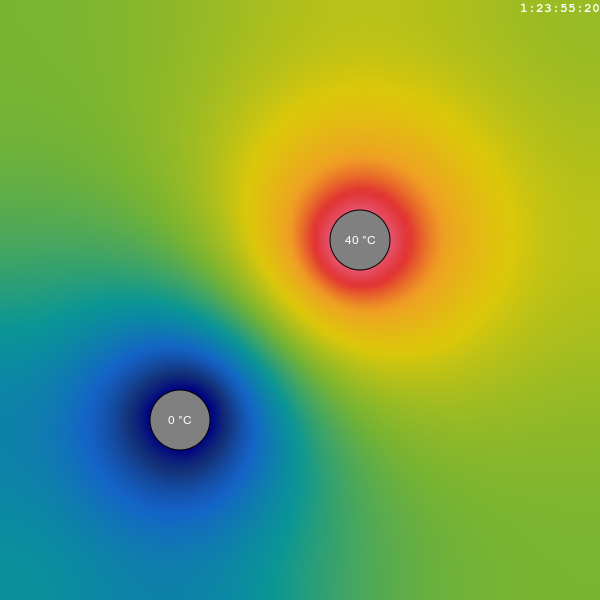
\includegraphics[width=.5\textwidth]{img/heatExample1}
\caption{Dystrybucja temperatury między dwoma punktami o różnych temperaturach}
\label{fig:heatExample1}
\end{figure}

\begin{figure}[!h]
\centering
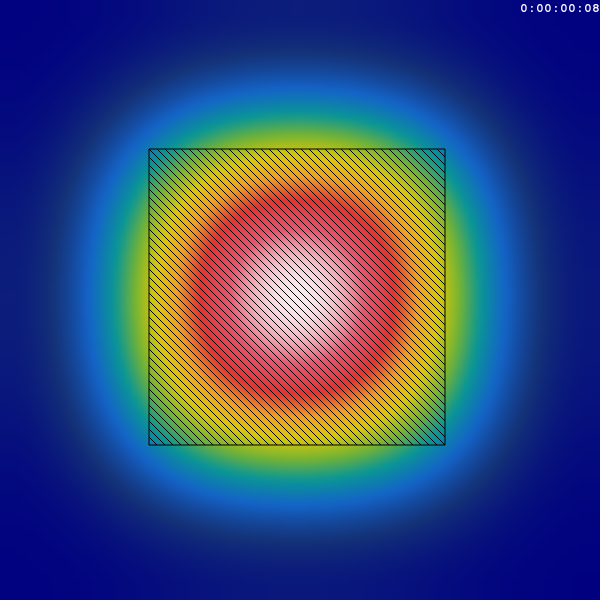
\includegraphics[width=.5\textwidth]{img/heatExample2}
\caption{Wymiana ciepła z otoczeniem i jej wpływ na dystrybucję temperatury 
w obiekcie}
\label{fig:heatExample2}
\end{figure}

\clearpage

\subsection{Silnik dynamiki płynów}

Drugi z silników fizycznych zajmuje się rozwiązywaniem równań związanych z
dynamiką płynów. Nie jest tak dokładny jak pierwszy, natomiast natomiast wyniki
są wystarczająco precyzyjne aby wizualnie zaprezentować wiele wartościowych
zjawisk fizycznych. Przede wszystkim używany jest do pokazywania konwekcji,
która odgrywa bardzo ważną rolę w procesie przekazywania energii cieplnej, ale
jako, że wymaga to obliczeń związanych z dynamiką płynów, także inne zjawiska z
tej dziedziny mogą być symulowane. Algorytm opiera się na rozwiązywaniu równania
Naviera-Stokesa (\ref{eq:fluid}) w następującej postaci:

\begin{equation}
\label{eq:fluid}
\frac{\partial \mathbf{v}}{\partial t}
= \alpha \nabla^2 \mathbf{v} - (\mathbf{v} \cdot \nabla) \mathbf{v} - \nabla p 
+ \mathbf{f}
\end{equation}

gdzie $\mathbf{v}$ to wektor prędkości, $\alpha$ to lepkość kinematyczna,
$p$ to ciśnienie, a $\mathbf{f}$ to zewnętrzna siła taka jak np. siła wyporu
lub grawitacji. Pierwsze wyrażenie po prawej stronie równania opisuje
dyfuzję pędu, a drugie adwekcje prędkości.

Prawo zachowania masy jest wymuszane przez warunek:
\begin{equation}
\nabla \cdot \mathbf{v} = 0
\end{equation}

Żeby dystrybucja temperatury w materiałach miała wpływ również na przepływ
otaczającego płynu (powietrza), w symulacji została uwzględniona wyporność
termiczna (jako siła zewnętrzna $\mathbf{f}$):

\begin{equation}
\mathbf{f}(x,y,z,t) = \gamma \left[ T(x,y,z,t) - T_0(x,y,t) \right] 
\mathbf{\vec{z}}
\end{equation}

gdzie $T_0(x,y,t)$ jest średnią temperaturą kolumny płynu w punkcie $(x,y)$
i czasie $t$, a $\gamma$ jest współczynnikiem ekspansji temperatury.

Równania, podobnie jak w przypadku poprzedniego silnika, zostały przekształcone
do postaci dyskretnej. Krok dyfuzji równania \ref{eq:fluid} jest rozwiązywany za
pomocą relaksacji tak jak w przypadku równania przewodnictwa cieplnego. Krok
adwekcji równania \ref{eq:fluid} jest rozwiązywany przy użyciu ze schematu
MacCormacka\footnote{Więcej informacji o metodzie MacCormacka:
\url{http://en.wikipedia.org/wiki/MacCormack_method}}. Dokładna analiza
wszystkich powyższych równań oraz ich przekształcenia umożliwiające stworzenie
finalnie zaimplementowanego algorytmu są przedstawione w autorskim opracowaniu
Charlesa Xie \cite{fluidEquation}. Rysunki \ref{fig:fluidExample1} oraz
\ref{fig:fluidExample2} prezentują rezultaty symulacji z wykorzystaniem
silnika dynamiki płynów.

\begin{figure}[!h]
\centering
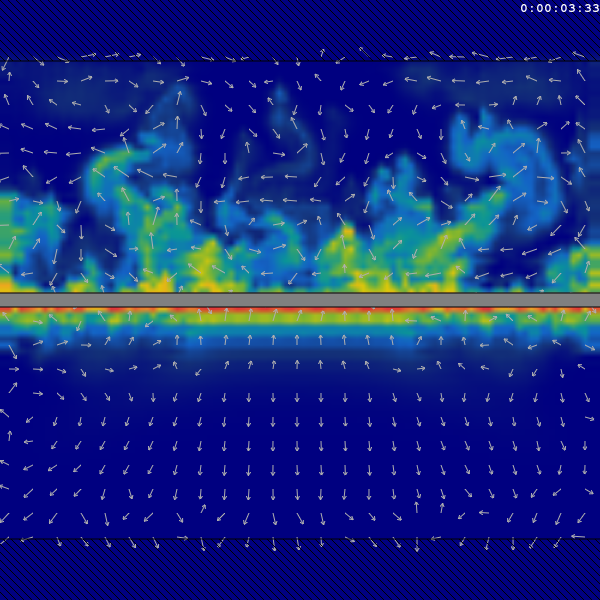
\includegraphics[width=.6\textwidth]{img/fluidExample1}
\caption{Rozgrzana płytka umieszczona w powietrzu, zjawisko konwekcji}
\label{fig:fluidExample1}
\end{figure}

\begin{figure}[!h]
\centering
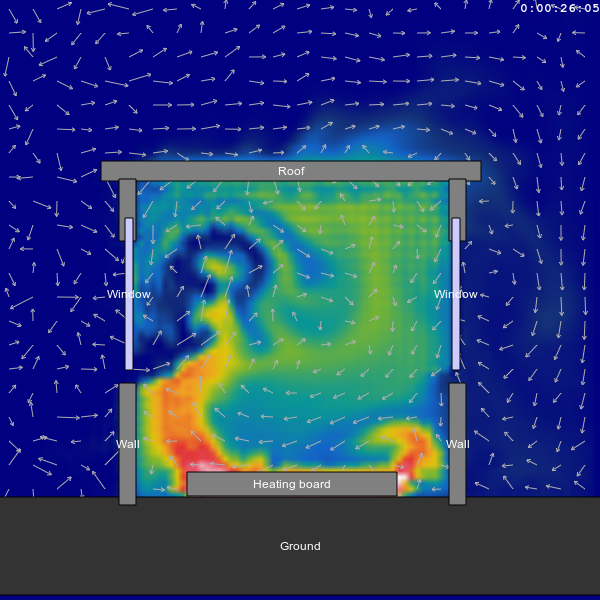
\includegraphics[width=.6\textwidth]{img/fluidExample2}
\caption{Naturalna konwekcja występująca w ogrzewanym pomieszczeniu oraz wpływ 
nieszczelności tego pomieszczenia na jej przebieg}
\label{fig:fluidExample2}
\end{figure}

\section{Podobne, istniejące rozwiązania}

Oczywiście narzędziem o bardzo podobnej funkcjonalności jest wspomniana
wcześniej wersja symulatora \en napisana w Javie, autorstwa Charlesa Xie. Jej
szczegółowy opis znajduje się w artykule \cite{orgEnergy2D}. Jednak kilka
czynników wyraźnie odróżnia pierwowzór od opisywanej w niniejszej pracy
aplikacji \en. Przede wszystkim są to:

\begin{itemize}

\item \textbf{Technologia implementacji oraz integracja ze środowiskiem
przeglądarki internetowej} -- pierwowzór używa technologii Java. Stąd wymaga aby
na komputerze użytkownika była zainstalowana wirtualna maszyna Java, a w
przypadku próby osadzenia symulacji w środowisku przeglądarki internetowej,
odpowiednie jej rozszerzenie. Wbrew pozorom, jest to dość problematyczne na
wielu szkolnych komputerach, które często są konfigurowane w najprostszy sposób,
a uczniowie ani nauczyciele nie mają praw administratora. Ponadto, nawet gdy te
wymagania są spełnione, sama integracja apletów Java ze stroną HTML jest
obarczona wieloma problemami.

Po pierwsze, jest to znacznie trudniejsze dla samych twórców zewnętrznych stron
internetowych w których ma zostać osadzona aplikacja. Aplety Javy nie są
naturalnym elementem stron HTML, dlatego nie można do nich zastosować technik
stylizacji i skalowania np. z użyciem popularnej technologii \ow{CSS} jak w
przypadku wersji \en napisanej w języku \js. Wiele programistów stron
internetowych nie jest też zaznajomiona z tą technologią, więc sama integracja
strony z apletem może być niedoskonała i spotkać się z niechętnym przyjęciem.
Aplikacja \en \js korzysta wyłącznie z technologii, które muszą być znane
każdemu programiście stron internetowych, stąd integracja jest bezproblemowa.

Z kolei dla użytkownika uciążliwe może być instalowanie i utrzymywanie
aktualnych wersji maszyny wirtualnej oraz rozszerzeń do przeglądarek. Ponadto,
aplet stanowi wyraźnie odrębną część strony internetowej, często też użytkownik
musi każdorazowo zezwolić na jego uruchomienie. Przez to wizualizacja może stać
się elementem pomijanym przez uczniów z powodu zwykłego zniechęcenia i znużenia.
Wykorzystanie w nowej wersji natywnych dla przeglądarki technologii, takich jak
\js oraz \ow{WebGL}, umożliwiło doskonałą, niezależną od żadnych zewnętrznych
technologii oraz działań użytkownika, integrację z dowolną stroną internetową.
Osadzona na stronie HTML aplikacja nie wymaga żadnych uciążliwych kroków aby
była widoczna, wygląda jak zwykły obrazek, jednak w rzeczywistości okazuje się
być zaawansowaną, interaktywną symulacją.

\item \textbf{Równoległe obliczenia wykonywane na karcie graficznej} --
pierwowzór zaimplementowany w języku Java umożliwia wyłącznie obliczenia
sekwencyjne na procesorze głównym, w przeciwieństwie do nowej wersji, która
korzystając z technologii \ow{WebGL}, umożliwia przeniesienie obliczeń
fizycznych na procesor karty graficznej. Zaowocowało to ogromnym wzrostem
wydajności, który szczegółowo jest analizowany w rozdziale
\ref{sec:testyWydajnosciowe}. Oryginalna wersja w Javie jest mocno ograniczona w
kwestiach szybkości działania symulacji, czyli szeroko pojętej interaktywności.

\item \textbf{Architektura, implementacja, funkcjonalność} -- ze względu na
powyższe różnice, rzeczą wspólną dla obu aplikacji są wyłącznie algorytmy
rozwiązujące równania fizyczne autorstwa Charlesa Xie. Wszystkie inne aspekty
tych dwóch programów różnią się od siebie, gdyż zupełnie różne są też założenia,
wybrane technologie oraz oczekiwane funkcjonalności.

\end{itemize}

Powyższe różnice tworzą nową jakość w przypadku aplikacji \en \js. Przede
wszystkim nowatorska, równoległa implementacja części algorytmów w nowoczesnej
technologii \ow{WebGL} może stanowić ciekawy wzór dla innych aplikacji, które
chciałby skorzystać z zysku jaki niesie równoległe wykonywanie obliczeń. Ze
względu na znacznie lepszą integrację ze środowiskiem przeglądarki internetowej,
nowa wersja ma szansę na znacznie lepsze rozpowszechnienie, docieranie do
użytkowników, a tym samym może mieć wyraźnie większy wpływ na zmianę oblicza
procesu edukacji.

W internecie można znaleźć również inne aplikacje \js, które prezentują różne
zjawiska i efekty fizyczne. Ze względu na wizualną atrakcyjność, często są to
również symulacje dynamiki płynów. Bardzo duży wkład w popularyzowanie takiego
wykorzystywania możliwości przeglądarek internetowych ma Evgeny Demidov. Na
swojej stronie \url{http://www.ibiblio.org/e-notes/webgl/gpu/contents.htm}
prezentuje liczne możliwe zastosowania języka \js oraz technologii \ow{WebGL}.
Znaczna część przykładów dotyczy fizyki, a nawet dynamiki płynów. W internecie
znaleźć można też inne dema prezentujące obliczenia mniej lub bardziej bazujące
na fizyce\footnote{Ciekawy zbiór aplikacji korzystających z technologii
\ow{WebGL}, w tym sporo aplikacji prezentujących zjawiska fizyczne, można
znaleźć na stronie Chrome Experiments: \url{http://www.chromeexperiments.com/}}.
Jednak te aplikacje, włącznie z przykładami Demidova, mają zdecydowanie inny
charakter niż aplikacja \en. Są znacznie mniejsze, oferują mniej możliwości
konfiguracji (często praktycznie w ogóle jej nie ma, gotowy jest wyłącznie jeden
przypadek) i nastawione są na prezentacje technologii, a nie skupiają się na
osiągnięciu konkretnego celu. \en posiada znacznie większą funkcjonalność i
tworzy złożoną, kompletną aplikację o jasno zdefiniowanym edukacyjnym
charakterze. Dlatego też zdecydowanie wyróżnia się na tle innych symulacji
fizycznych napisanych w \js, nawet jeśli wykorzystują one technologię \ow{WebGL}
(co wciąż jest podejściem bardzo rzadko spotykanym i nowatorskim).
